% ==========================================
% MoE Kernel Optimizations & Performance
% ==========================================

\begin{block}{MoE Kernel Optimization Journey}
We benchmarked our progressively optimized Mixture-of-Experts implementations at DeepSeek-V3 scale ($E=256, EL=32, D=7168$, $K=8$) to evaluate NVIDIA B200 hardware utilization mapping across sequences ($T \in \{64, 256, 512, 1024, 2048, 4096\}$).

\vspace{0.5em}
\textbf{Key Optimizations (Blackwell Architecture):}
\begin{itemize}
    \item \textbf{Naive Baseline:} Computes routing and FFN as explicit kernel launches per expert ($O(E)$ dispatches). Thrashing $L2$ and completely unscalable past $T=1024$.
    \item \textbf{Opt 1 (Tiled GEMM):} Natively leverages Shared Memory (\texttt{smem}) overlapping across GEMM tile accumulations to cut DRAM trips.
    \item \textbf{Opt 2 (Fused Routing):} Collapses Softmax, probability distributions, top-k gate index retrieval, and logit computations entirely onto the Register File before touching main memory.
    \item \textbf{Opt 3 (Grouped-GEMM):} Radically transforms the workload from $O(E)$ sequential loops to constant $O(1)$ massive HW dispatches. Sorts sequences efficiently and natively balances execution tiles across SMs.
    \item \textbf{Opt 4 (Double-Buffered Async DMA):} Bypasses Register Files utilizing \texttt{\_\_pipeline\_memcpy\_async} instructions. Maps 64x64 math structures concurrently across 8 active warps leveraging Tensor Cores.
    \item \textbf{DeepSeek-V3 (Production):} Differs materially from \texttt{Opt4} by utilizing the Sigmoid+Bias un-softmaxed grouping selection natively. It injects a highly parallel vectorized memory-layout execution loop, excising routing delays directly down by a further 30\% from \texttt{Opt4}!
\end{itemize}
\vspace{0.5em}

\textbf{Latency Scaling Across Implementations (in milliseconds)}
\begin{table}[]
\begin{tabular}{lrrrrrr}
\textbf{Implementation} & \textbf{T=64} & \textbf{T=256} & \textbf{T=512} & \textbf{T=1024} & \textbf{T=2048} & \textbf{T=4096} \\
\midrule
Naive Baseline  & 220.55 & 824.51 & 1628.77 & 3254.86 & 6698.64 & 13401.07 \\
Opt 1 (Tiled GEMM) & 166.61 & 670.30 & 1307.72 & 2622.22 & 5331.44 & 10860.38 \\
Opt 2 (Fused Routing)& 166.49 & 665.59 & 1332.42 & 2628.35 & 5333.88 & 10859.67 \\
Opt 3 (Grouped-GEMM)& 7.31 & 26.02 & 45.07 & 88.72 & 181.22 & 394.34 \\
Opt 4 (Dbl-Buf) & 1.36 & 4.10 & 7.89 & 15.43 & 30.44 & 60.58 \\
\midrule
\textbf{DeepSeek-V3} & \textbf{1.59} & \textbf{2.08} & \textbf{1.67} & \textbf{4.42} & \textbf{5.68} & \textbf{10.23} \\
\end{tabular}
\end{table}

\vspace{0.5em}
\textbf{Throughput Scaling Across Implementations (Tokens/sec)}
\begin{table}[]
\begin{tabular}{lrrrrrr}
\textbf{Implementation} & \textbf{T=64} & \textbf{T=256} & \textbf{T=512} & \textbf{T=1024} & \textbf{T=2048} & \textbf{T=4096} \\
\midrule
Naive Baseline & 290 & 310 & 314 & 315 & 306 & 306 \\
Opt 1 (Tiled GEMM) & 384 & 382 & 392 & 391 & 384 & 377 \\
Opt 2 (Fused Routing)& 384 & 385 & 384 & 390 & 384 & 377 \\
Opt 3 (Grouped-GEMM)& 8,756 & 9,838 & 11,361 & 11,542 & 11,301 & 10,387 \\
Opt 4 (Dbl-Buf) & 47,036 & 62,380 & 64,867 & 66,375 & 67,285 & 67,616 \\
\midrule
\textbf{DeepSeek-V3} & \textbf{40,287} & \textbf{123,054} & \textbf{306,251} & \textbf{231,781} & \textbf{360,436} & \textbf{400,403} \\
\end{tabular}
\end{table}

\vspace{1em}
\begin{figure}[h]
    \centering
    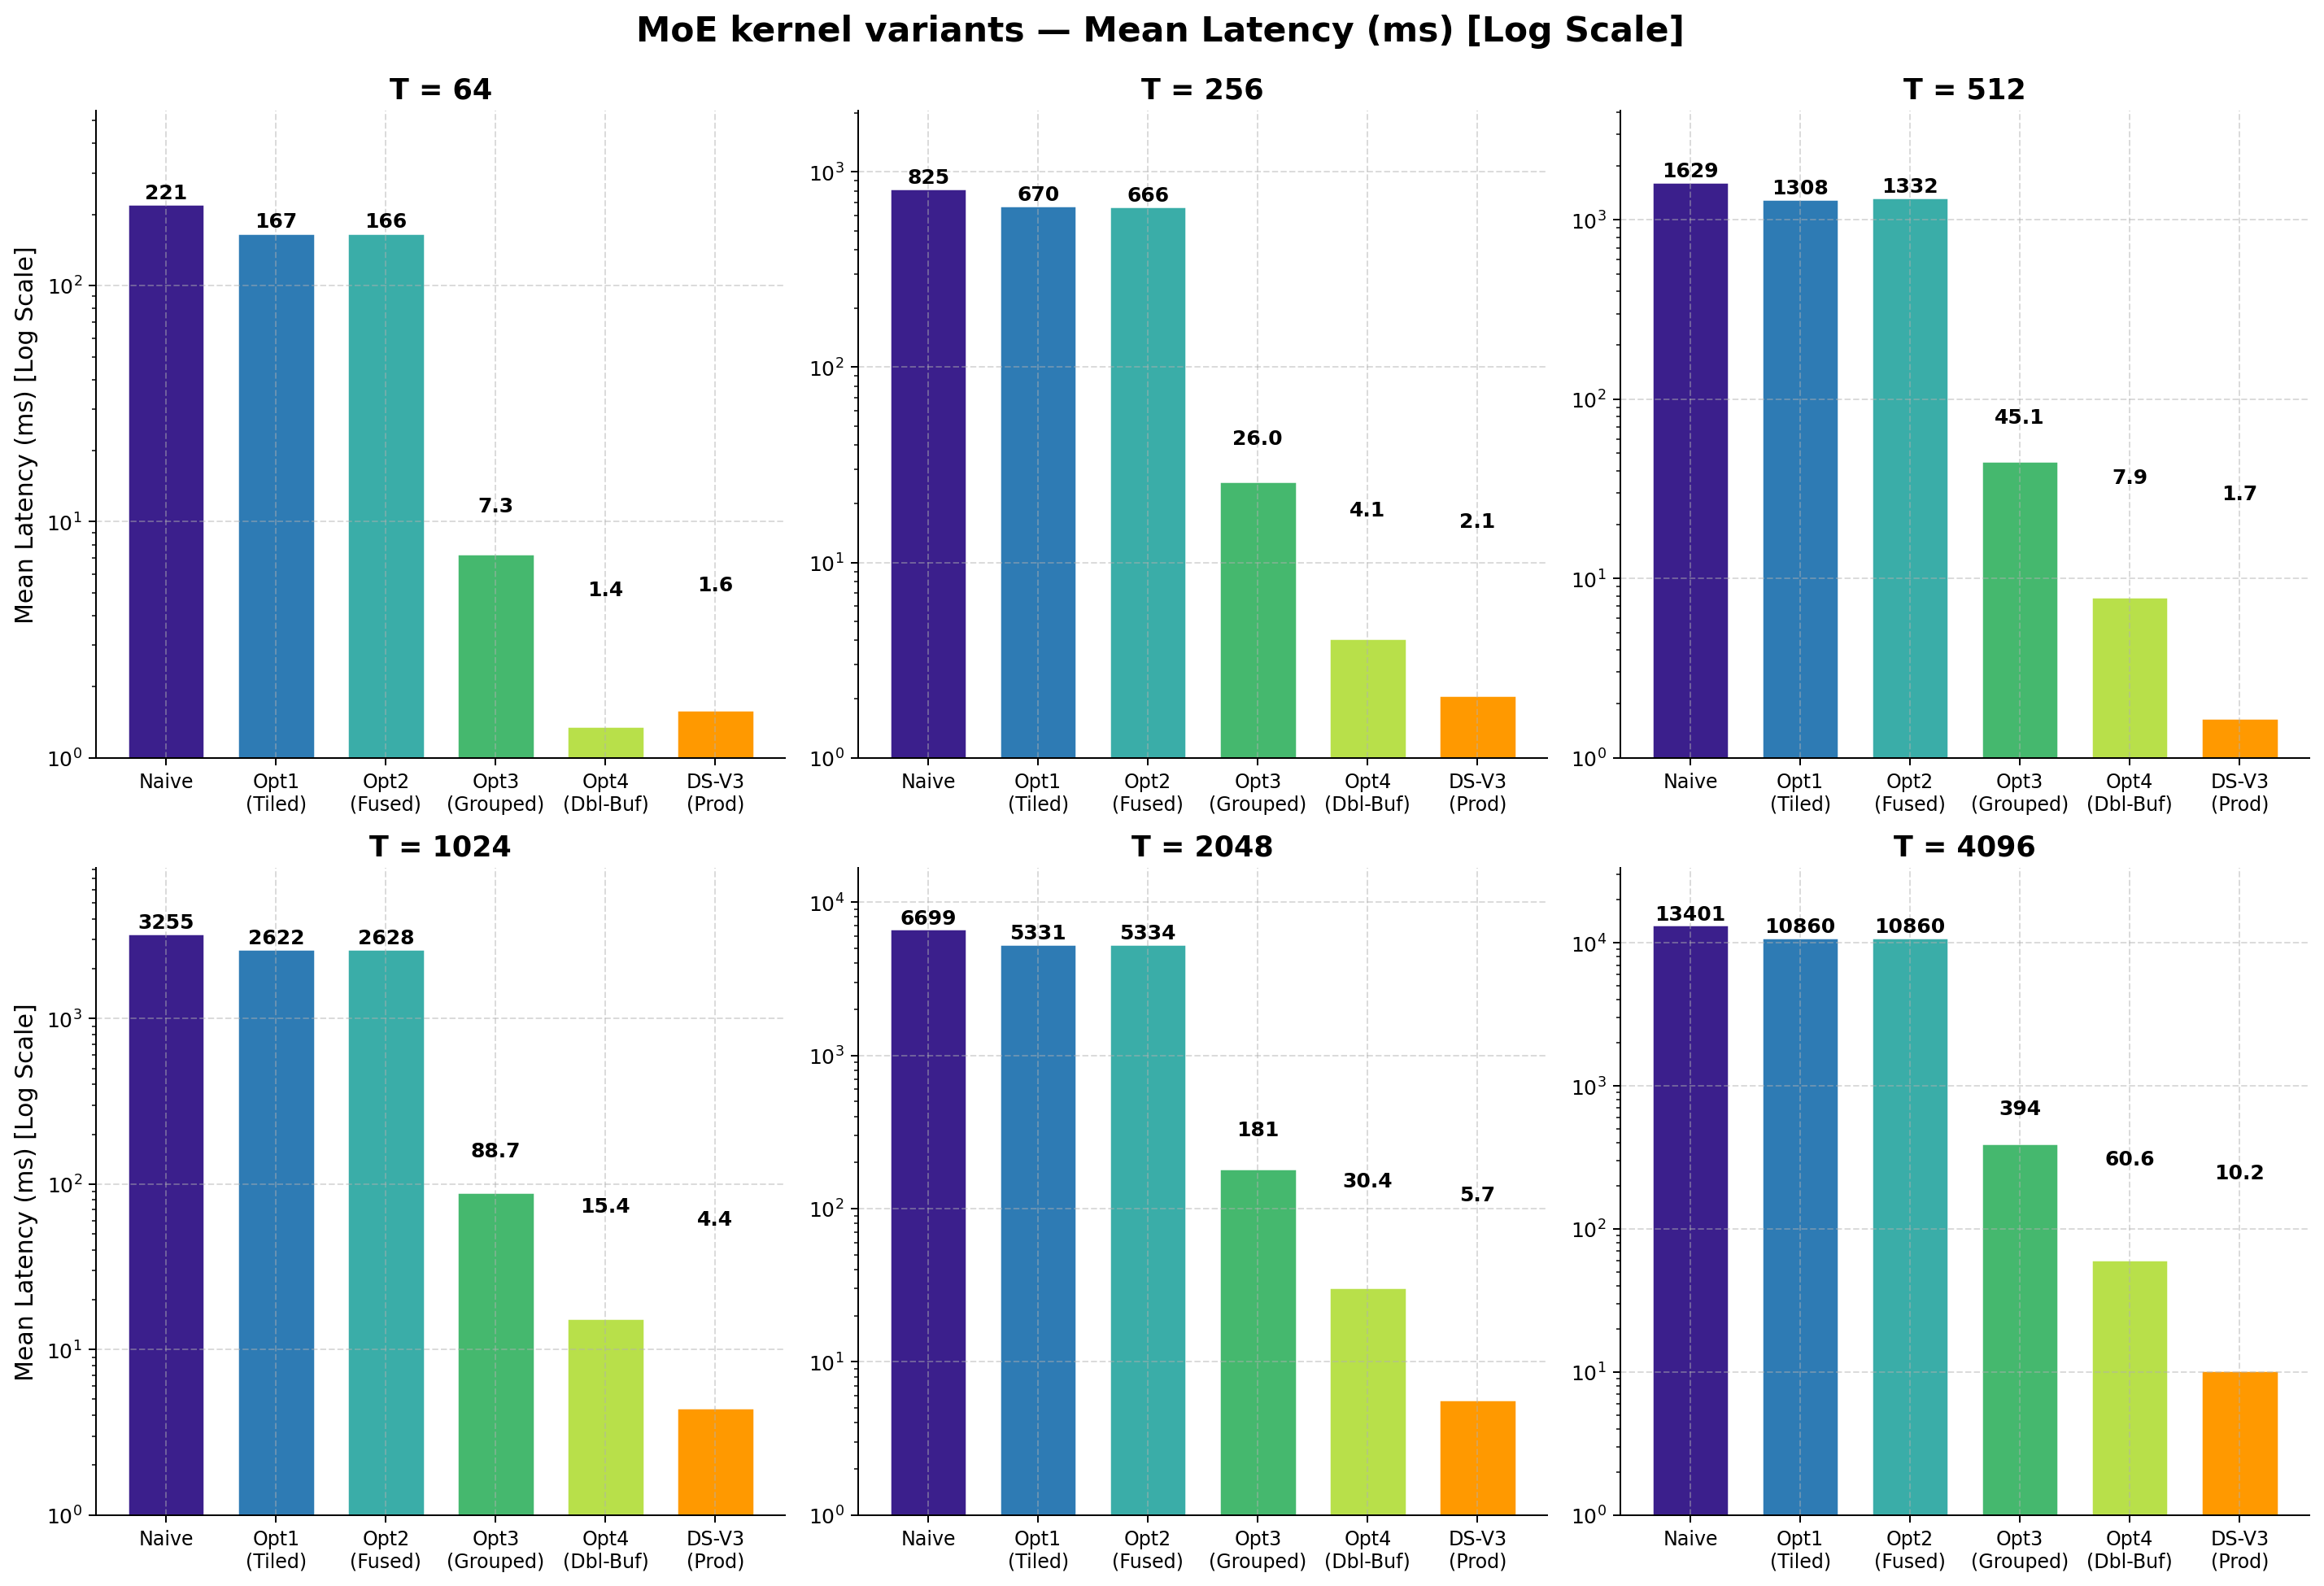
\includegraphics[width=0.95\linewidth]{figures/moe_latency_seqlen.png}
    \caption{MoE Latency (ms) progression across sequence lengths. Logarithmic scale visualizes the 1000x gap from baseline.}
\end{figure}

\begin{figure}[h]
    \centering
    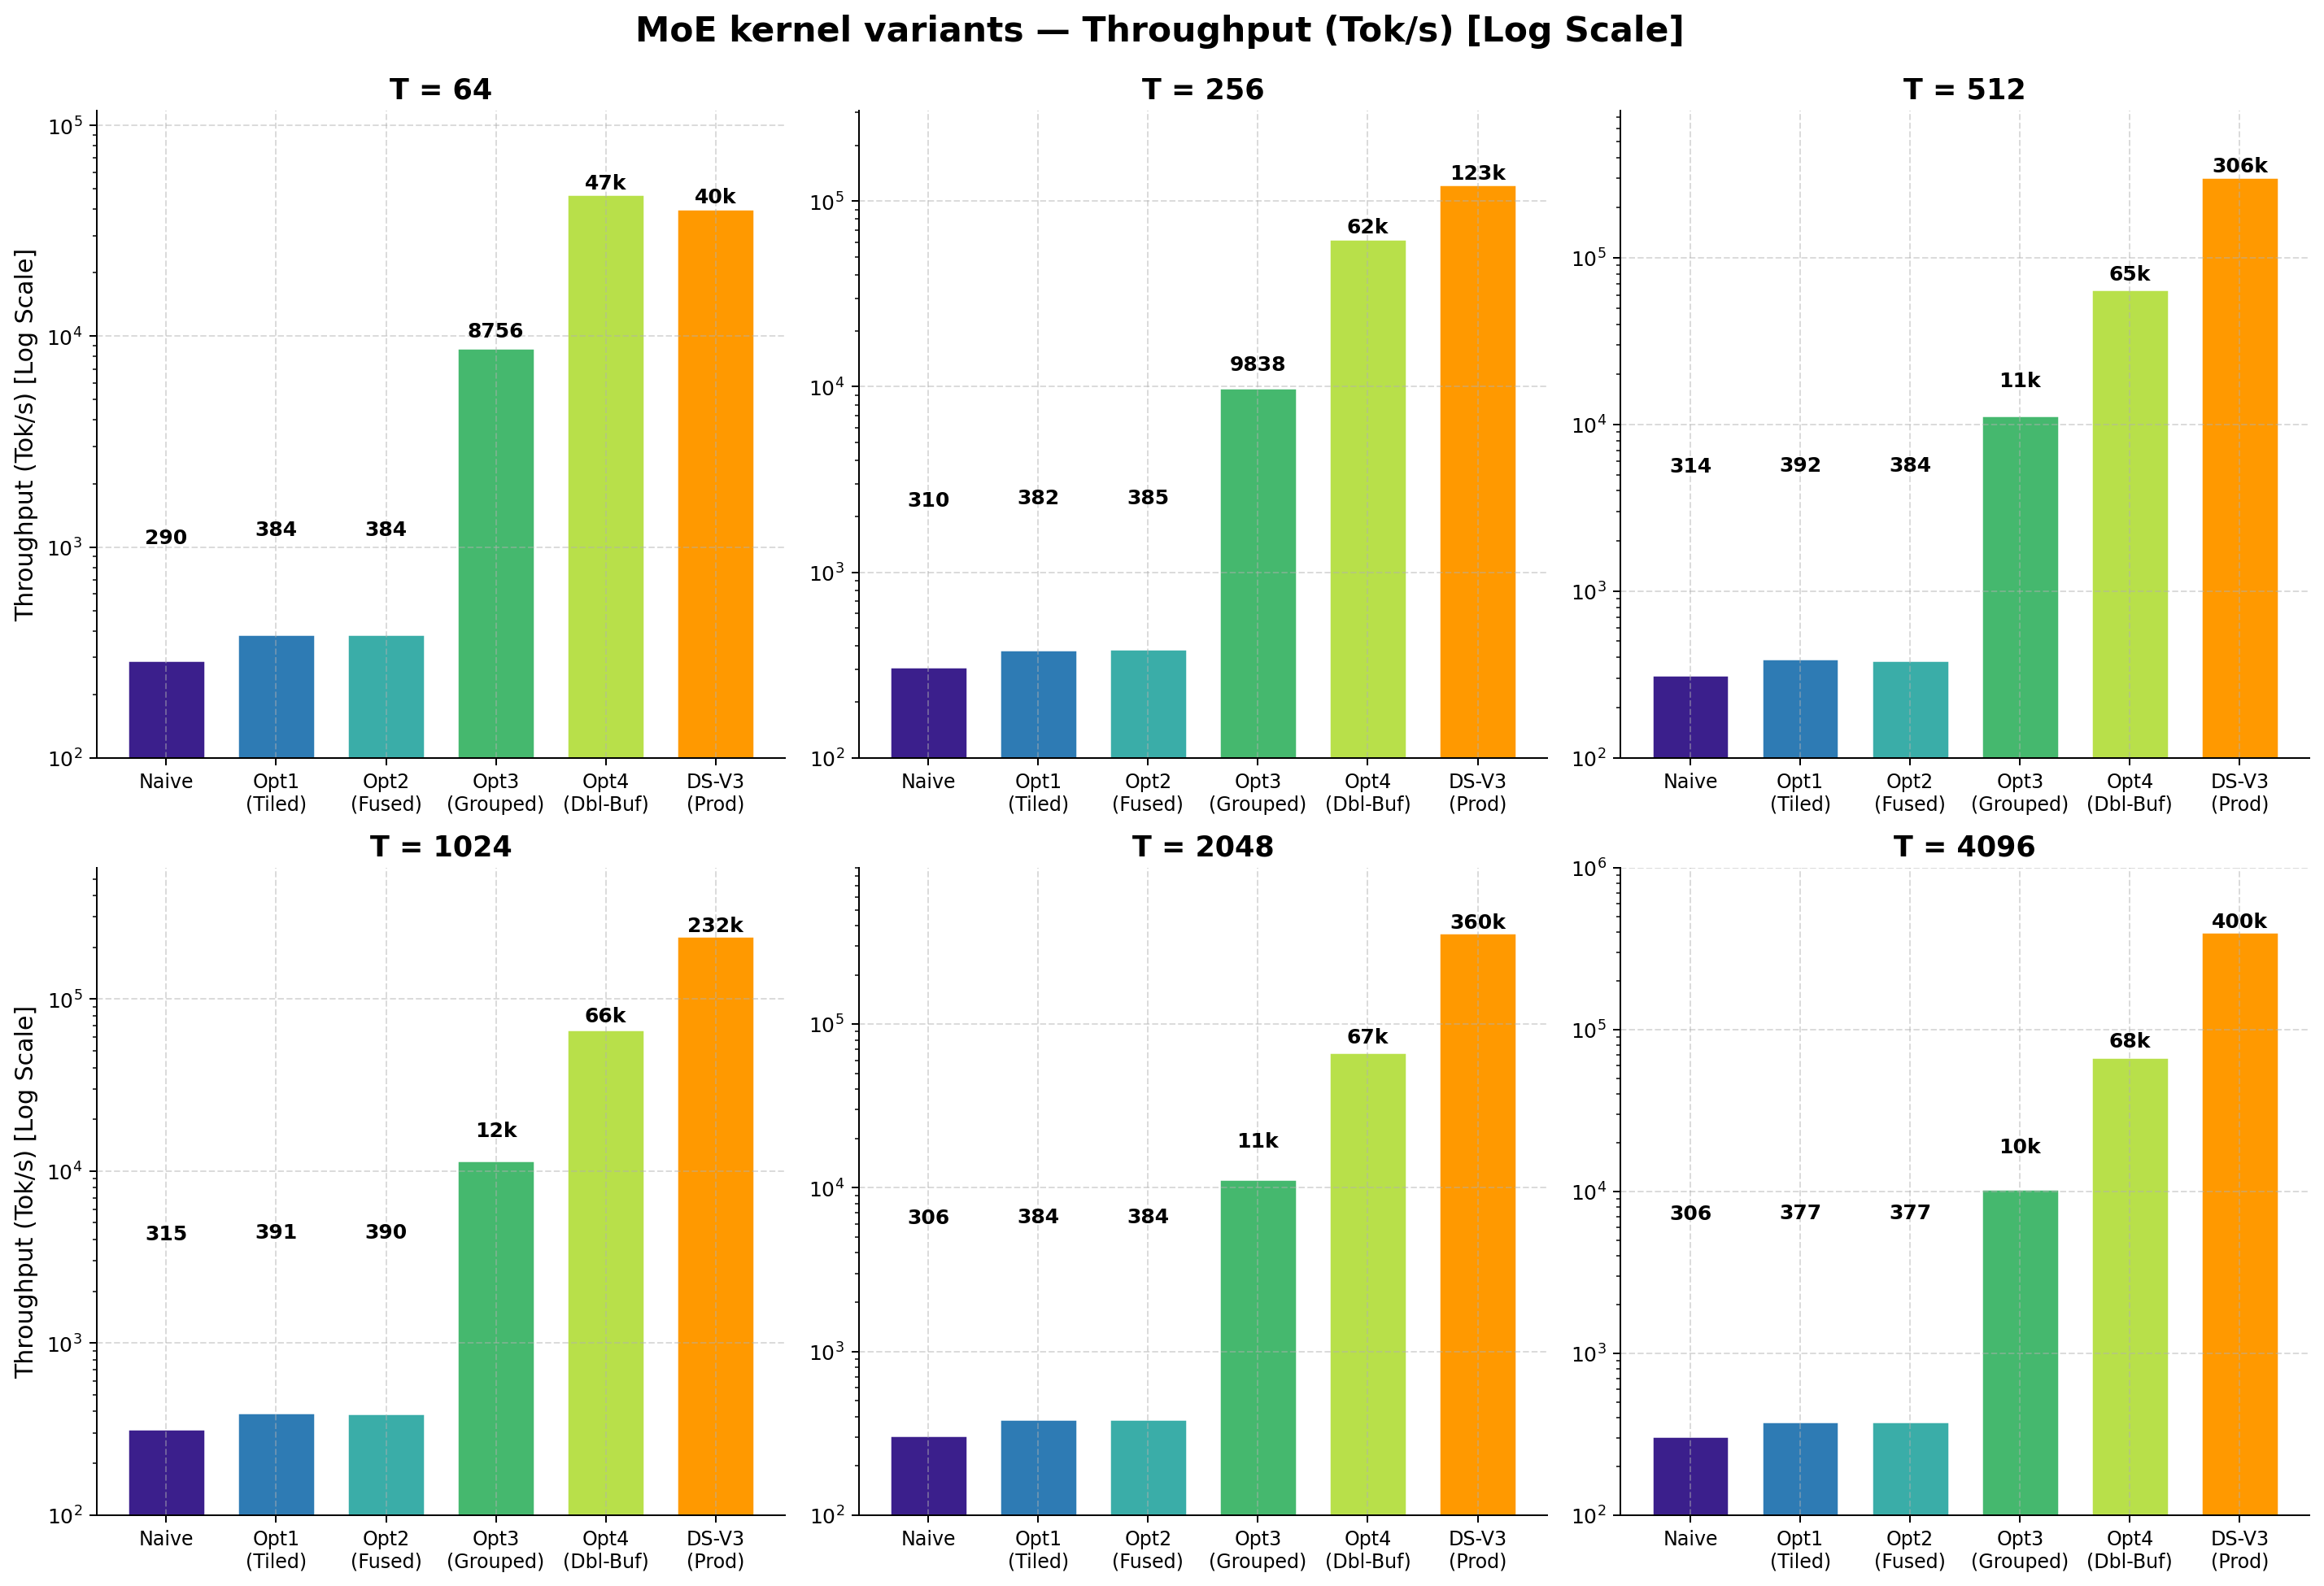
\includegraphics[width=0.95\linewidth]{figures/moe_throughput_seqlen.png}
    \caption{MoE Throughput (Tokens/s) progression across sequence lengths. Logarithmic scale showcases the immense Tensor Core saturation of DeepSeek-V3 at boundaries.}
\end{figure}
\end{block}
